%!TEX TS-program = xelatex

% Официальный шаблон презентации НИУ ВШЭ в beamer (LaTeX)
% Версия 2.0
% Язык — русский   
% Автор шаблона - Данил Фёдоровых (fedorovykh@gmail.com)

%%% Для корректной работы шаблона необходима 
%%% установка в систему бесплатного шрифта HSE Sans
%%% https://www.hse.ru/info/brandbook/#font

\documentclass[aspectratio=169]{beamer}

\newbool{russian}
\booltrue{russian}  % Загружает русскоязычный логотип ВШЭ
\usepackage{HSE-theme/beamerthemeHSE} % Подгружаем тему

%%% Работа с русским языком и шрифтами
\usepackage[english,russian]{babel}   % загружает пакет многоязыковой вёрстки
\usepackage[no-math]{fontspec}      % подготавливает загрузку шрифтов Open Type, True Type и др.
	\setsansfont{Arial} 
	\setmonofont{Courier New}
\usepackage{mathspec}
	%(Digits,Latin,Greek)[Numbers={Lining,Proportional}]{HSE Sans}
	\setmathrm[Numbers={Lining,Proportional}]{Arial}
\uselanguage{russian}
\languagepath{russian}
\deftranslation[to=russian]{Theorem}{Теорема}
\deftranslation[to=russian]{Definition}{Определение}
\deftranslation[to=russian]{Definitions}{Определения}
\deftranslation[to=russian]{Corollary}{Следствие}
\deftranslation[to=russian]{Fact}{Факт}
\deftranslation[to=russian]{Example}{Пример}
\deftranslation[to=russian]{Examples}{Примеры}

\usepackage{blindtext} 		% Случайный текст
\graphicspath{{images/}}  	% Папка с картинками

%%% Информация об авторе и выступлении
\title[Заголовок]{Реализация и сравнительный анализ оптимизированных алгоритмов Краскалла и Прима} 
\subtitle{Курсовая работа}
\author[Имя автора]{Работу выполнил: Турсунов Данил Вячеславович \\ Научный руководитель: Малышев Дмитрий Сергеевич}
\institute{Образовательная программа "Фундаментальная математика"}
\date{\today}

\begin{document}	% Начало презентации

\frame[plain]{\titlepage}	% Титульный слайд

\begin{frame}
\frametitle{Цели и задачи работы}
	\hspace{0.5cm} В данной курсовой работе будет рассматриваться задача построения минимального остовного дерева по заданному связному неориентированному взвешенному графу.
\end{frame}

\begin{frame}
	\frametitle{Теоретическая часть}
	\framesubtitle{Часть 1}
	\begin{definition}
		Для связного неориентированного графа \( G = (V, E) \) остовное дерево \( T = (V, E') \) --- это граф, удовлетворяющий условиям:
		\par 1) \( T \) является \textit{деревом},
		\par 2) \( V(T) = V(G) \) (содержит все вершины исходного графа),
		\par 3) \( E' \subseteq E \) (рёбра принадлежат исходному графу).
	\end{definition}
\end{frame}

\begin{frame}
	\frametitle{Теоретическая часть}
	\framesubtitle{Часть 2}
	\begin{definition}
		Для взвешенного связного неориентированного графа $G$ минимальное остовное дерево --- это остовное дерево $T \subseteq G$, такое что сумма весов рёбер $T$ минимальна среди всех возможных остовных деревьев.
	\end{definition}
\end{frame}

\begin{frame}
	\frametitle{Теоретическая часть}
	\framesubtitle{Часть 3}
	\hspace{0.5cm} Курсовая работа представляет собой написание программы (кода), которая состоит из 2-х частей: алгоритмической и аналитической. Изначально запускается алгоритмическая часть кода, которая написана на языке программирования C++, в ней реализованы следующие подпрограммы:
	
	\hspace{0.5cm}- алгоритм Краскалла;
	
	\hspace{0.5cm}- оптимизация алгоритма Краскалла;
	
	\hspace{0.5cm}- алгоритм Прима;
	
	\hspace{0.5cm}- оптимизация алгоритма Прима;
	
	\hspace{0.5cm}- генератор графов;
	
	\hspace{0.5cm}- итоговая подпрограмма, которая генерирует графы различного количества вершин и рёбер и запускает на них алгоритмы Краскалла и Прима, замеряя время построения минимального остовного поддерева и выводя в отдельные файлы (для каждой пропорции количества рёбер и количества вершин создаётся отдельный файл) количество вершин и время построения.
\end{frame}

\begin{frame}
	\frametitle{Теоретическая часть}
	\framesubtitle{Часть 4}
	\hspace{0.5cm}Далее запускается аналитическая часть, состоящая из двух подпрограмм, каждая из которых берёт информацию из файлов, сгенерированных алгоритмической частью:
	
	\hspace{0.5cm}- программа, проводящая сравнительный анализ скорости работы алгоритмов Краскалла и Прима. Она строит отдельный график времени, потребовавшегося на построение минимального остовного дерева, в зависимости от количества вершин для каждой пропорции количества рёбер и количества вершин;
	
	\hspace{0.5cm}- программа, строящая графики отношения времени выполнения алгоритмов Краскалла и Прима к оценке их алгоритмической сложности.
\end{frame}

\begin{frame}
	\frametitle{Алгоритм Краскалла}
	\framesubtitle{Часть 1}
	\hspace{0.5cm}В алгоритме Краскалла минимальное остовное дерево строится поэтапно, путём добавления ребёр исходного графа к графу без рёбер, от минимального к максимальному, в случае, если это ребро соединяет вершины, принадлежащие разным компонентам связности строящегося графа.
\end{frame}

\begin{frame}
	\frametitle{Пример работы алгоритма Краскалла}
	\framesubtitle{Часть 1}
	\begin{figure}[htbp]
		\centering
		\	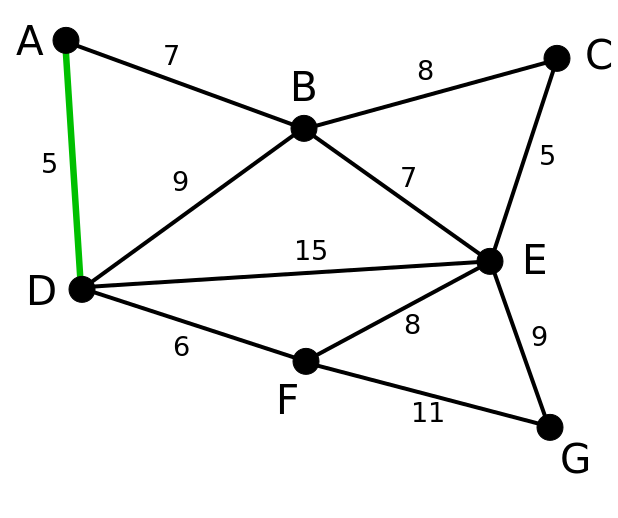
\includegraphics[width=0.6\textwidth]{images/example_kruskal/kruskal_1.png}
	\end{figure}
\end{frame}

\begin{frame}
	\frametitle{Пример работы алгоритма Краскалла}
	\framesubtitle{Часть 2}
	\begin{figure}[htbp]
		\centering
		\	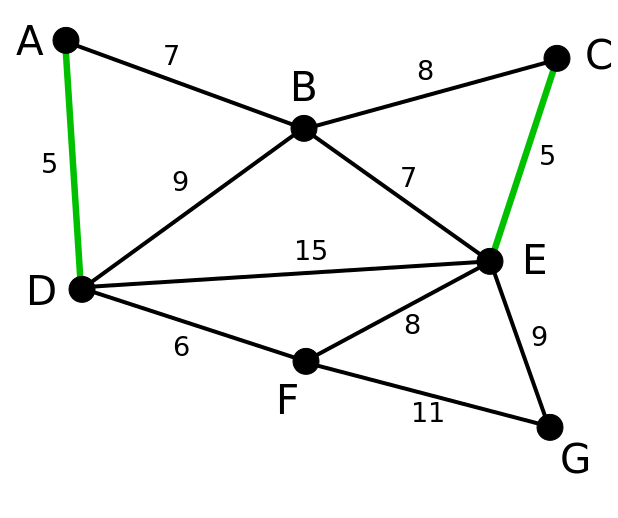
\includegraphics[width=0.6\textwidth]{images/example_kruskal/kruskal_2.png}
	\end{figure}
\end{frame}

\begin{frame}
	\frametitle{Пример работы алгоритма Краскалла}
	\framesubtitle{Часть 3}
	\begin{figure}[htbp]
		\centering
		\	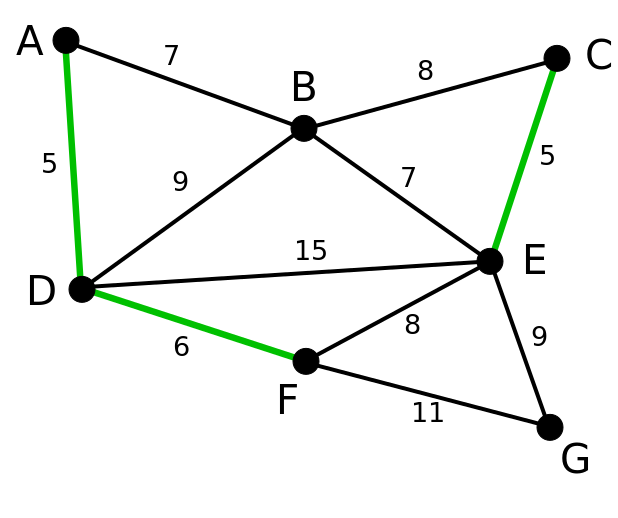
\includegraphics[width=0.6\textwidth]{images/example_kruskal/kruskal_3.png}
	\end{figure}
\end{frame}

\begin{frame}
	\frametitle{Пример работы алгоритма Краскалла}
	\framesubtitle{Часть 4}
	\begin{figure}[htbp]
		\centering
		\	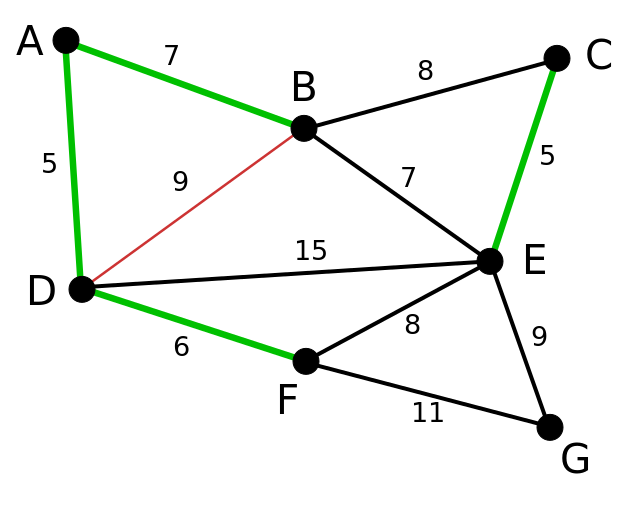
\includegraphics[width=0.6\textwidth]{images/example_kruskal/kruskal_4.png}
	\end{figure}
\end{frame}

\begin{frame}
	\frametitle{Пример работы алгоритма Краскалла}
	\framesubtitle{Часть 5}
	\begin{figure}[htbp]
		\centering
		\	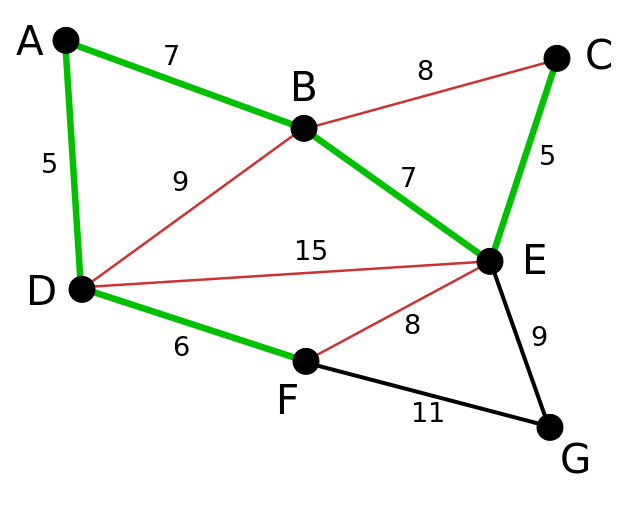
\includegraphics[width=0.6\textwidth]{images/example_kruskal/kruskal_5.png}
	\end{figure}
\end{frame}

\begin{frame}
	\frametitle{Пример работы алгоритма Краскалла}
	\framesubtitle{Часть 6}
	\begin{figure}[htbp]
		\centering
		\	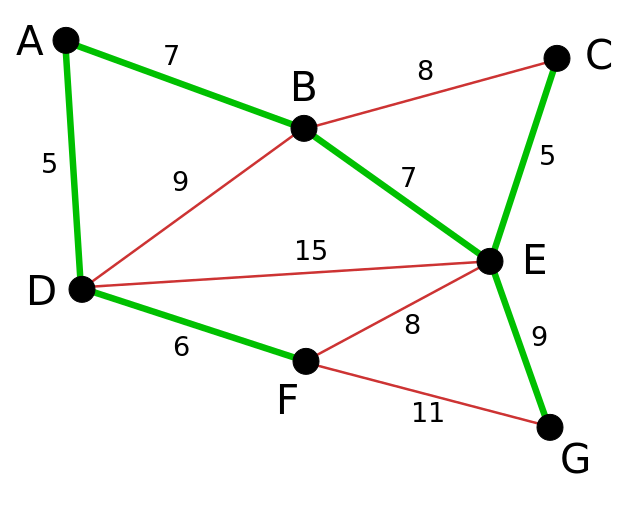
\includegraphics[width=0.6\textwidth]{images/example_kruskal/kruskal_6.png}
	\end{figure}
\end{frame}

\begin{frame}
	\frametitle{Оптимизация алгоритма Краскалла}
	\framesubtitle{Часть 1}
	\hspace{0.5cm}В описании алгоритма Краскалла был упущен момент, связанный в проверкой двух вершин на то, соединены ли вершины путём или нет. Для проверки этого факта используется структура данных, называемая системой непересекающихся множеств.
\end{frame}

\begin{frame}
	\frametitle{Оптимизация алгоритма Краскалла}
	\framesubtitle{Часть 2}
	\hspace{0.5cm}Система непересекающихся множеств представляет собой множество вершин, указывающих на своего предка. То есть, по сути, конкретное множество представляет собой иерархическую структуру, дерево, корнем которого является вершина-представитель множества. Это сделано для того, чтобы множества можно было объединить, указав у вершины-представителя предка (другими словами, подвесив вершину-представителя к другой), который является членом другого множества (необязательно представителем)
\end{frame}

\begin{frame}
	\frametitle{Оптимизация алгоритма Краскалла}
	\framesubtitle{Часть 3}
	\hspace{0.5cm}Таким образом, для объединения множеств двух вершин необходимо:
	
	\hspace{0.5cm}1) найти вершины-представителей множеств этих двух вершин;
	
	\hspace{0.5cm}2) подвесить вершину-представителя одного множества к вершине-представителю другого множества.
\end{frame}

\begin{frame}
	\frametitle{Оптимизация алгоритма Краскалла}
	\framesubtitle{Часть 4}
	\hspace{0.5cm}В алгоритмической части программы СНМ реализована как класс DSU, у которого есть 2 метода: метод find\_parent и метод unite, которые ищут вершину-представителя конкретной вершины и объединяют множества двух вершин (необязательно представителей) соответственно.
\end{frame}

\begin{frame}
	\frametitle{Оптимизация алгоритма Краскалла}
	\framesubtitle{Часть 5}
	\hspace{0.5cm}В методе find\_parent на вход принимается вершина, далее идёт подъём по её предкам вплоть до того момента, когда у вершины не будет предка, а, значит, она является корнем дерева и вершиной-представителем. Соответственно, метод возвращает вершину-представителя.
\end{frame}

\begin{frame}
	\frametitle{Оптимизация алгоритма Краскалла}
	\framesubtitle{Часть 6}
	\hspace{0.5cm}Метод unite принимает на вход 2 вершины, находит у них вершины-представителей и подвешивает одну вершину представителя к другому.
\end{frame}

\begin{frame}
	\frametitle{Оптимизация алгоритма Краскалла}
	\framesubtitle{Часть 7}
	\hspace{0.5cm}Однако, с такой реализацией скорость объединения множеств может становиться линейной, превращая итоговую скорость работы алгоритма в квадратичную. Для более быстрого объединения будем пользоваться эвристическими подходами.
\end{frame}

\begin{frame}
	\frametitle{Оптимизация алгоритма Краскалла}
	\framesubtitle{Часть 8}
	\hspace{0.5cm}Первая эвристика заключается в подвешивании менее глубокого дерева к более глубокому. При таком подходе глубина дерева не увеличится (значит, и не увеличится скорость поиска вершины-представителя), кроме случая, когда глубина обоих деревьев одинакова. Для внедрения этой эвристики в программу придётся хранить глубину дерева.
\end{frame}

\begin{frame}
	\frametitle{Оптимизация алгоритма Краскалла}
	\framesubtitle{Часть 9}
	\hspace{0.5cm}Вторая эвристика заключается в том, чтобы обновлять предка у вершин, через которые мы прошли при поиске вершины представителя. Будем запоминать, через какие вершины мы прошли и, когда дойдём до вершины представителя, подвесим все вершины к вершине-представителю, сокращая таким образом маршрут между вершиной и вершиной-представителем в будущем. При таком подходе глубина перестанет подсчитываться точно и станет оценкой глубины сверху.
\end{frame}

\begin{frame}
	\frametitle{Оптимизация алгоритма Краскалла}
	\framesubtitle{Часть 10}
	\hspace{0.5cm}После внедрения эвристик в программе, множества будут объединяться практически мгновенно, оценка сложности будет равняться \( O(\alpha(n)) \), где \( \alpha(n) \) - обратная функция Аккермана (настолько медленно растёт, что можно принять за константу).
\end{frame}

\begin{frame}
	\frametitle{Алгоритм Прима}
	\framesubtitle{Часть 1}
	\hspace{0.5cm}В алгоритме Прима минимальное остовное дерево строится жадно, путём поэтапного добавления рёбер к строящемуся дереву. Очередное добавленное ребро выбирается минимальным из тех, кто соединяет дерево с вершинами, в дерево ещё не добавленные.
\end{frame}

\begin{frame}
	\frametitle{Пример работы алгоритма Прима}
	\framesubtitle{Часть 1}
	\begin{figure}[htbp]
		\centering
		\	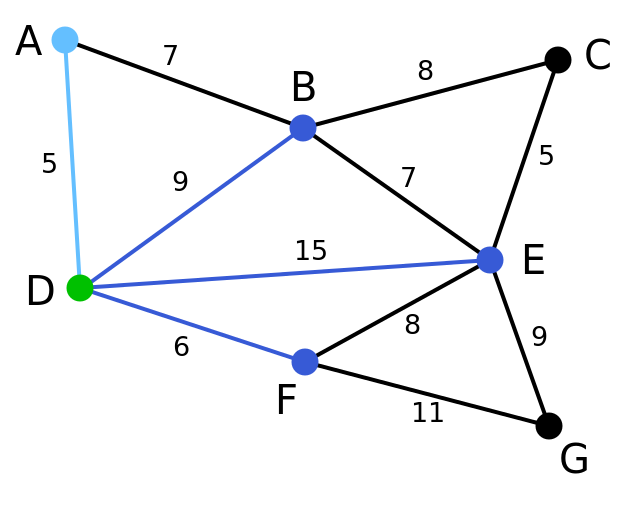
\includegraphics[width=0.6\textwidth]{images/example_prim/prim_1.png}
	\end{figure}
\end{frame}

\begin{frame}
	\frametitle{Пример работы алгоритма Прима}
	\framesubtitle{Часть 2}
	\begin{figure}[htbp]
		\centering
		\	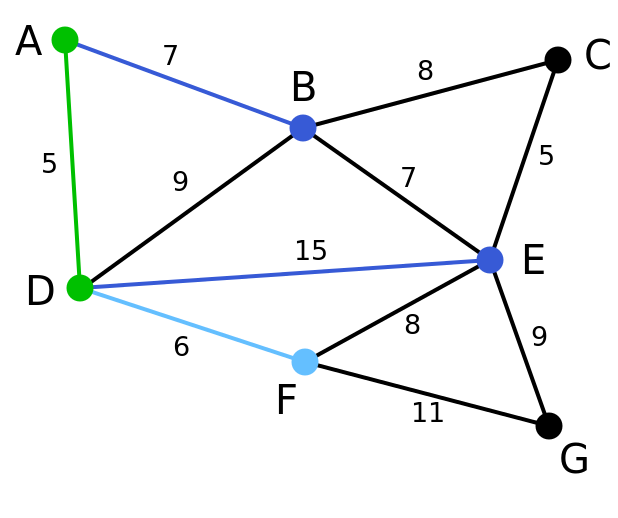
\includegraphics[width=0.6\textwidth]{images/example_prim/prim_2.png}
	\end{figure}
\end{frame}

\begin{frame}
	\frametitle{Пример работы алгоритма Прима}
	\framesubtitle{Часть 3}
	\begin{figure}[htbp]
		\centering
		\	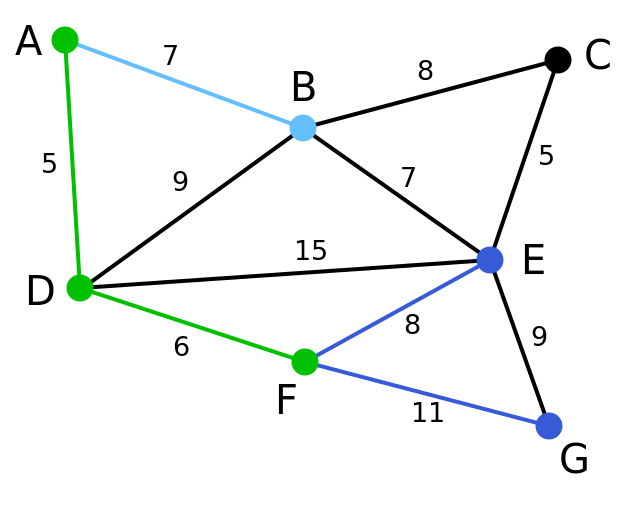
\includegraphics[width=0.6\textwidth]{images/example_prim/prim_3.png}
	\end{figure}
\end{frame}

\begin{frame}
	\frametitle{Пример работы алгоритма Прима}
	\framesubtitle{Часть 4}
	\begin{figure}[htbp]
		\centering
		\	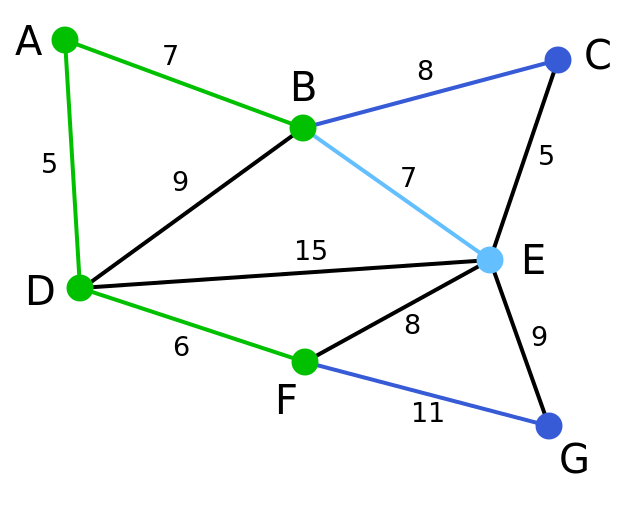
\includegraphics[width=0.6\textwidth]{images/example_prim/prim_4.png}
	\end{figure}
\end{frame}

\begin{frame}
	\frametitle{Пример работы алгоритма Прима}
	\framesubtitle{Часть 5}
	\begin{figure}[htbp]
		\centering
		\	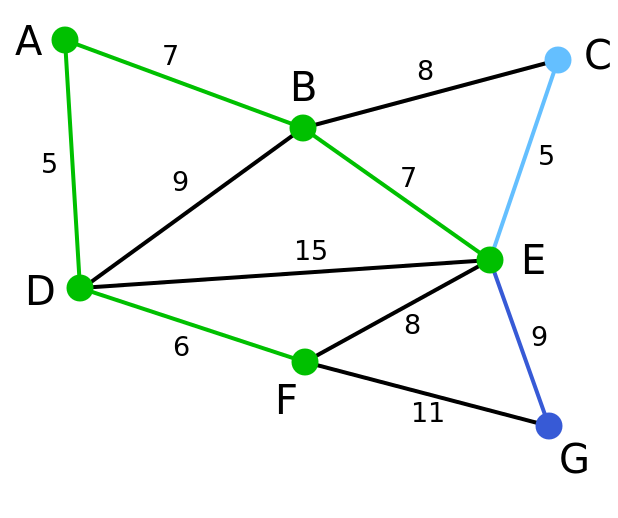
\includegraphics[width=0.6\textwidth]{images/example_prim/prim_5.png}
	\end{figure}
\end{frame}

\begin{frame}
	\frametitle{Пример работы алгоритма Прима}
	\framesubtitle{Часть 6}
	\begin{figure}[htbp]
		\centering
		\	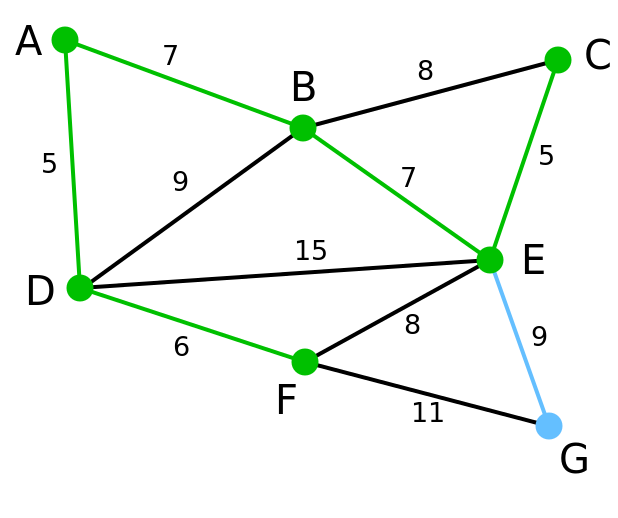
\includegraphics[width=0.6\textwidth]{images/example_prim/prim_6.png}
	\end{figure}
\end{frame}

\begin{frame}
	\frametitle{Пример работы алгоритма Прима}
	\framesubtitle{Часть 7}
	\begin{figure}[htbp]
		\centering
		\	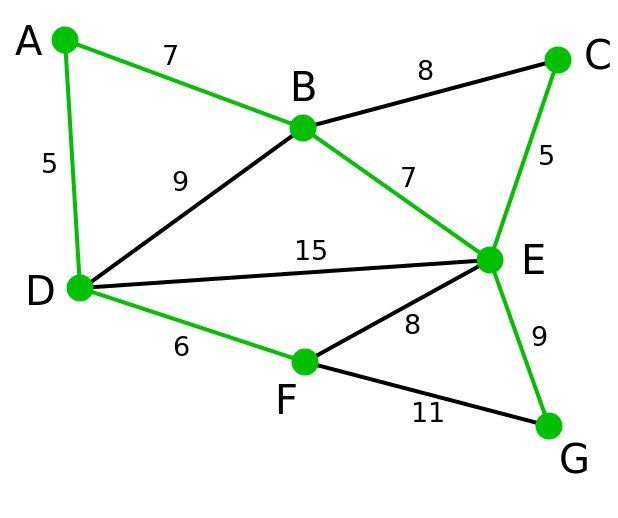
\includegraphics[width=0.6\textwidth]{images/example_prim/prim_7.png}
	\end{figure}
\end{frame}

\begin{frame}
	\frametitle{Оптимизация алгоритма Прима}
	\framesubtitle{Часть 1}
	\hspace{0.5cm}В главе выше умышленно был упущен момент выбора очередной вершины, которую планируется добавить в строящееся дерево.
	\hspace{0.5cm}Тривиальный алгоритм этой процендуры состоит в том, чтобы циклом пройтись по всем ещё не добавленным вершинам и посмотреть все их рёбра, найти среди них то ребро, что соединяет текущую вершину с деревом, и является минимальным среди таких рёбер, то есть просто запомнить минимальное ребро.
\end{frame}

\begin{frame}
	\frametitle{Оптимизация алгоритма Прима}
	\framesubtitle{Часть 2}
	\hspace{0.5cm}Очевидно, что этот алгоритм в худшем случае пройдётся по всем вершинам и по всем рёбрам, что превращает алгоритм Прима в квадратичный относительно количества вершин и рёбер, поэтому в реализованном алгоритме используется оптимизация, основанная на очереди с приоритетами.
\end{frame}

\begin{frame}
	\frametitle{Оптимизация алгоритма Прима}
	\framesubtitle{Часть 3}
	\hspace{0.5cm}Очередь с приоритетами - структура данных, которая является бинарным деревом с одним свойством - значения в вершинах меньше, чем значения в потомках (или больше, чем значения предков). С таким свойством очередь с приоритетами отождествляется с кучей минимумов, в дальнейшем будем использовать именно такой термин.
\end{frame}

\begin{frame}
	\frametitle{Оптимизация алгоритма Прима}
	\framesubtitle{Часть 4}
	\hspace{0.5cm}Куча минимумов позволяет находить минимальное значение практически моментально, в нашем случае, будем находить минимальное ребро, удовлетворяющее условиям. В программе куча минимумов реализована как класс, обладающий полями и методами. Реализована очередь с приоритетами в программе не как дерево, а как список, где поиск левого или правого ребёнка, а также предка, осуществляется по индексам \( 2i + 1 \), \( 2i + 2 \), \( (i - 1)/2 \), где i - индекс текущей вершины соответственно.
\end{frame}

\begin{frame}
	\frametitle{Оптимизация алгоритма Прима}
	\framesubtitle{Часть 5}
	\hspace{0.5cm}Для кучи минимумов реализованы следующие методы: добавление элемента (он не более чем за \( O(log~n) \) займёт нужное место в структуре данных), удаление элемента (тоже занимает \( O(log~n) \)), а также метод, позволяющий узнать минимальный элемент в куче за \( O(1) \). Помимо этого реализованы методы, благодаря которым работают перечисленные выше методы, являющиеся публичными в смысле объектно-ориентированного программирования.
\end{frame}

\begin{frame}
	\frametitle{Оптимизация алгоритма Прима}
	\framesubtitle{Часть 6}
	\hspace{0.5cm}Вернёмся к алгоритму Прима. В цикле, где происходит поиск очередной вершины, вызывается функция find\_min, которая возвращает подходящую вершину. Эта функция принимает на вход кучу минимумов, состоящую из соседних строящемуся дереву рёбер, и берёт рёбра из этой кучи одно за другим до тех пор, пока не найдёт ребро, соединяющее ещё не использованную вершину с деревом, это ребро и будет являться минимальным среди таких.
	\hspace{0.5cm}При таком подходе итоговая сложность работы алгоритма Прима будет \( O((n + m) log~n) \).
\end{frame}

\begin{frame}
	\frametitle{Генерация графов для сравнительного анализа}
	\framesubtitle{Часть 1}
	\hspace{0.5cm}Генерация графов происходит следующим образом: все вершины соединяются рёбрами, образуя круг. Далее случайно выбирается 2 вершины, и, если нет рёбер, соединяющих эти 2 вершины, то ребро добавляется. Если же ребро уже есть, то ещё раз выбираем случайно 2 вершины и проделываем ту же процедуру, и так до тех пор, пока ребро не будет добавлено. Этот алгоритм повторяется, пока не будет добавлено необходимое количество рёбер.
\end{frame}

\begin{frame}
	\frametitle{Сравнительный анализ алгоритмов Прима и Краскалла}
	\framesubtitle{Часть 1}
	\begin{figure}[htbp]
		\centering
		\
		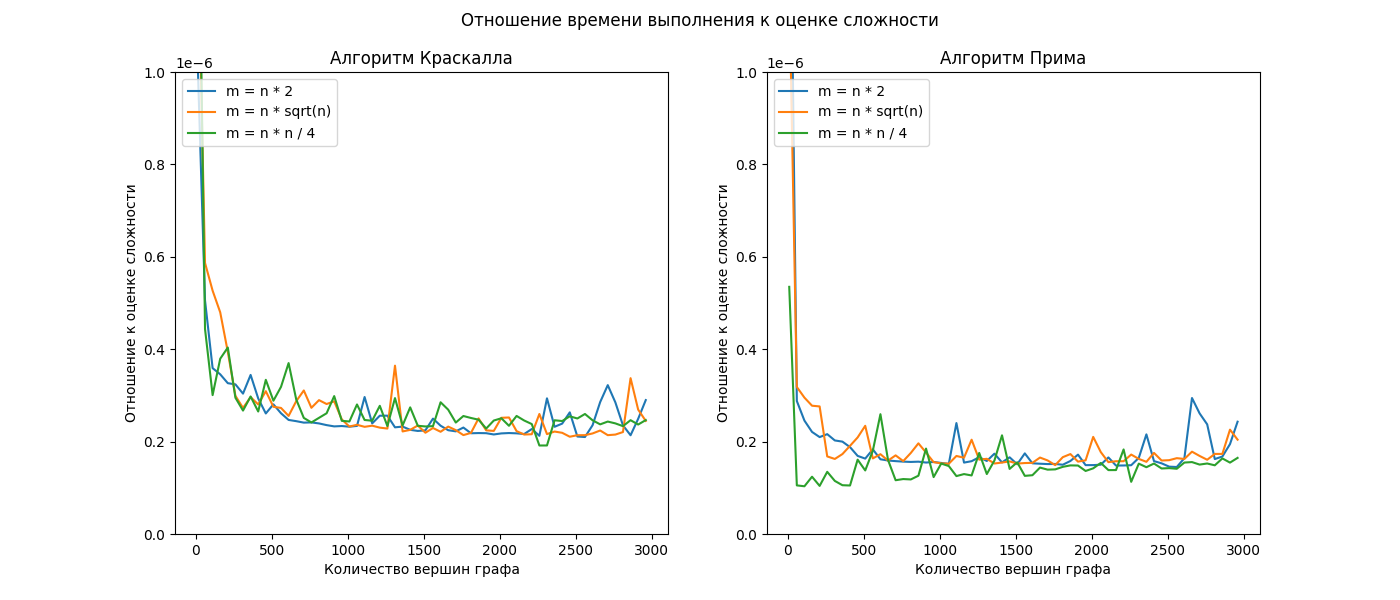
\includegraphics[width=1\textwidth]{images/big_o_analysis.png}
	\end{figure}
\end{frame}

\begin{frame}
	\frametitle{Сравнительный анализ алгоритмов Прима и Краскалла}
	\framesubtitle{Часть 2}
	\begin{figure}[htbp]
		\centering
		\	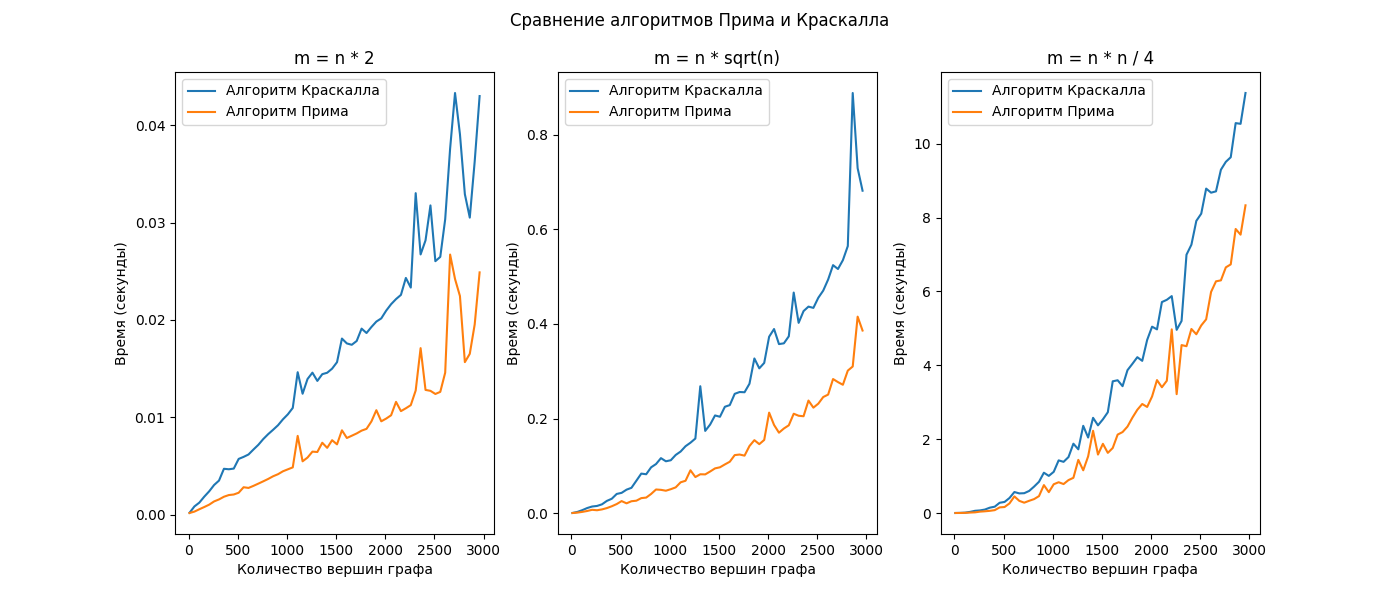
\includegraphics[width=1\textwidth]{images/algorithm_comparasion.png}
	\end{figure}
\end{frame}

\begin{frame}
\frametitle{Ссылка на репозиторий в GitHub}
	\hspace{0.5 cm}Реализация алгоритмов Краскалла и Прима на языке программирования C++ и код, необходимый для их сравнительного анализа, на языке программирования Python находятся в открытом репозитории на GitHub по следующей ссылке:
	\href{https://github.com/dan1lka257/coursework_3}{\textcolor{blue}{\underline{github.com/dan1lka257/coursework\_3}}}
\end{frame}

\begin{frame}
	\frametitle{Список литературы}
	\begingroup
	\renewcommand{\section}[2]{}
	\begin{thebibliography}{10}
		\bibitem{boruvka1926}
		Borůvka O. 
		\textit{O jistém problému minimálním}. 
		Práce Moravské Přírodovědecké Společnosti, 1926. 
		Vol. 3, No. 3, pp. 37--58.
		
		\bibitem{kruskal_history}
		Иванов А. В. 
		\textit{К истории двух знаменитых оптимизационных алгоритмов в теории графов}. 
		История науки и техники, 2015.
		
		\bibitem{elibrary1}
		Петров С. К. 
		\textit{Алгоритмы Прима и Крускала: сравнительный анализ}. 
		Журнал вычислительной математики, 2018.
		
		\bibitem{okhotin2024}
		Охотин А. 
		\textit{Лекция 2: Алгоритмы на графах}. 
		2024.
		
		\bibitem{elibrary2}
		Сидоров М. Н. 
		\textit{Применение алгоритмов Прима и Крускала в сетевых структурах}. 
		Информационные технологии, 2020.
		
		\bibitem{cormen2009}
		Cormen T. H., Leiserson C. E., Rivest R. L., Stein C. 
		\textit{Introduction to Algorithms}. 
		3rd ed. MIT Press, 2009.
		
	\end{thebibliography}
	\endgroup
\end{frame}

\end{document}